\documentclass[a4paper]{scrartcl}
\usepackage[utf8]{inputenc}
\usepackage[english]{babel}
\usepackage{graphicx}
\usepackage{lastpage}
\usepackage{pgf}
\usepackage{wrapfig}
\usepackage{fancyvrb}
\usepackage{fancyhdr}
\usepackage{hyperref}
\pagestyle{fancy}

\catcode`\_=\active
\protected\def_#1_{\textit{#1}}

% Create header and footer
\headheight 27pt
\pagestyle{fancyplain}
\lhead{\footnotesize{Network Programming, ID1212}}
\chead{\footnotesize{Web services}}
\rhead{}
\lfoot{}
\cfoot{\thepage}
\rfoot{}

% Create title page
\title{Assignment 4 - Web services}
\subtitle{Network Programming, ID1212}
\author{Bernardo Gonzalez Riede, begr@kth.se}
\date{\today}

\begin{document}

\maketitle

%Introduction
\section{Introduction}
Goals:
\begin{itemize}
	\item Develop a three-tier web-based application using frameworks
	\item Deploy and run a web-based application on an application server.
\end{itemize}


%Literature
\section{Literature Study}
As in previous assignments, the main source were the video lectures on the topic and the example code.

%Literature
\section{Method}
As in previous assignments, the mvc approach has been used again to layer the program.

The choice for a database fell on MySQL because of past works with it.
The implementation was realized in Netbeans in Java 8 EE using Pyara as the application server.


\section{Result}

Link to public Github repository with code:
\href{https://github.com/MemBernd/ID1212-Web-services}{https://github.com/MemBernd/ID1212-Web-services}

\subsection{Layering}
The layering of the application is divided into four layers:
\begin{itemize}
	\item The _view_ holds the JSF page.
	\item The _controller_ is used as a EJB.
	\item The _model_ holds the JPA entities.
	\item The _storage_ is responsible for connecting to the MySQL database.
\end{itemize}


%subsection covering persistent storage stuff
\subsection{Database}
The database in \ref{fig:database} consists of two tables.
The first table acts as a catalog, holding the different currencies, while the second one is the result of a many to many association of the catalog to itself.

\begin{figure}[h!]
  \begin{center}
    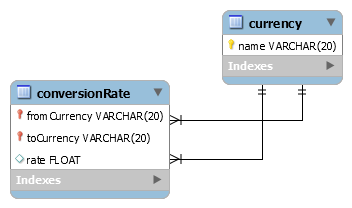
\includegraphics[scale=0.8]{db.png}
    \caption{Table relations in database.}
    \label{fig:database}
  \end{center}
\end{figure}



%subsection covering rmi stuff
\subsection{Frameworks}

\subsubsection{JSF}
Being a JSF, view.CurrencyConverter has mostly getters and setters (l. 52 - 118) for several private variables.
The JSF annotations are in line 22 \& 23, namely the name and the scope.


Some of the variables from the JSF are injected dynamically in converter.xhtml. A few use a conditional (e. g. converter.xhtml l. 32) to be rendered only if their value is different from 0, as to not show these values at the first loading of the page.




\subsubsection{EJB}
EJB related annotations in controller.Controller are found in line 22 \& 23.
Here, the EJB runs every method in a new transaction and is _stateless_.
It contains two methods:
\begin{enumerate}
	\item listCurrencies() (l. 31) to list all available currencies, e.g. to populate the comboboxes.
	\item convert() (l. 39) to do the actual conversion.
\end{enumerate}


\subsubsection{JPA}
After the database had been created, the automated process in netbeans to create entities from an existing database has been used to create the three entities in the model layer.

The entities corresponding to a table, i.e. _Currency_ and _Conversionrate_, include named queries in the beginning of their files (between lines 25 to 30). 
One of them is used in storage.CurrencyDAO line 33 to find all available currencies.
In the same file on line 40, the model is used directly to find a certain primary key, i.e. a combination of _from_ and _to_ currency.

The model is accessed through an EntityManager (l. 28 \& 29). Line 28 references the persitence unit defined in _persistence.xml_.



\subsection{Client side}
The user can access the application through a browser, which presents him with the jsf (see \ref{fig:ui}).
The user is able to select between 4 currencies to convert between them.
In case he selects the same currency, the application will return, hence show, the same amount as entered.

\begin{figure}[h!]
  \begin{center}
    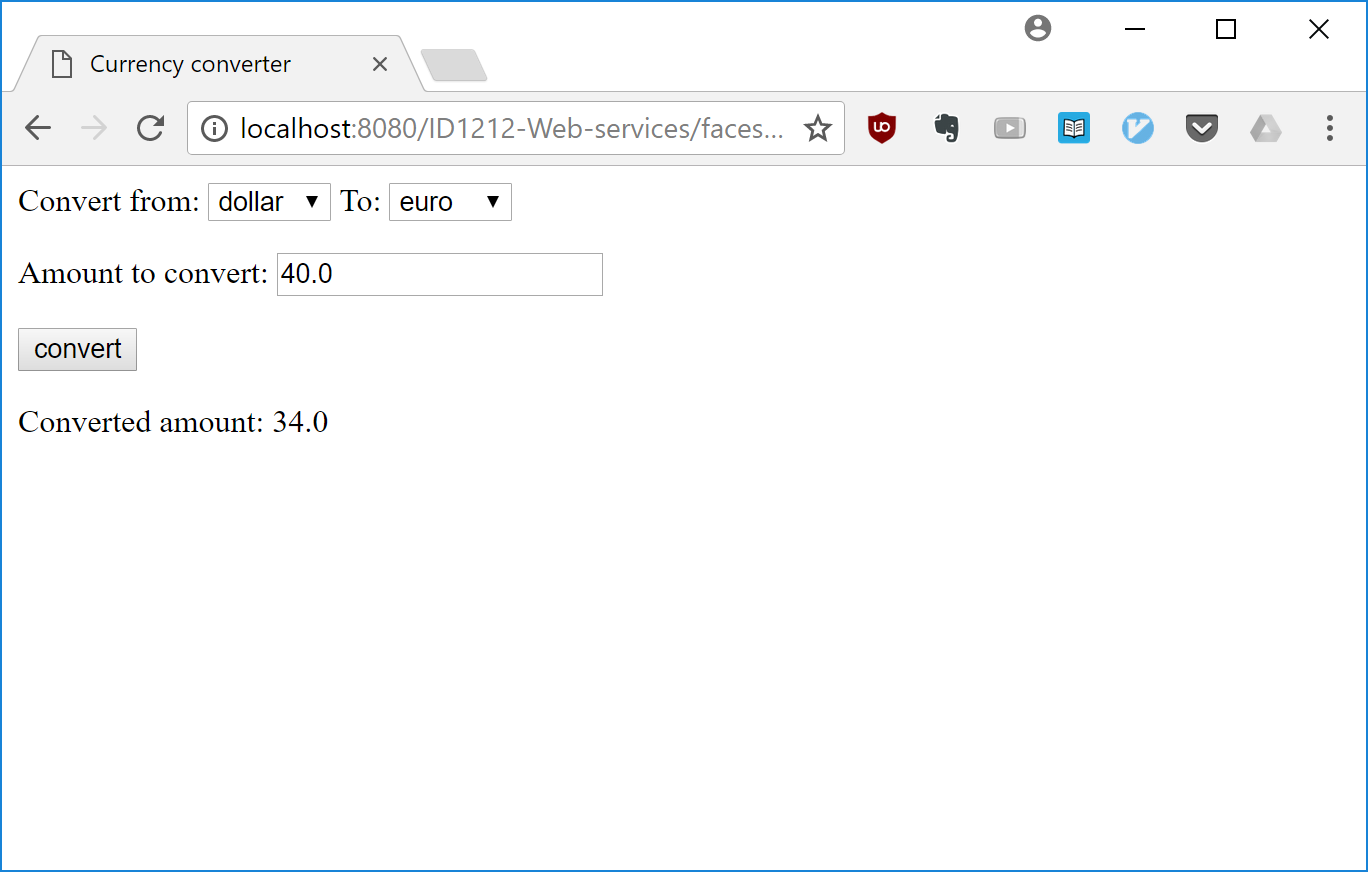
\includegraphics[scale=0.5]{ui.png}
    \caption{Browser interface}
    \label{fig:ui}
  \end{center}
\end{figure}

%subsection discussion
\section{Discussion}
Through the use of comboboxes the incorrect input is limited to the use of non digits in the currency amount.
Through the use of Beans, this behaviour is captured instantly and the user is shown a message similar to:
\\_ 'XX' must be a number consisting of one or more digits._

%subsection comments
\section{Comments About the Course}

It took almost 9 hours to complete this assignment.
\begin{itemize}
        \item 1 hour 37 min for coding.
        \item 4 hours 6 min for the report.
        \item 3 hours 13 min watching videos, taking notes and thinking about how to tackle the problem.
\end{itemize}




\end{document}
